
%%%%%%%%%%%%%%%%%%%%%%% file typeinst.tex %%%%%%%%%%%%%%%%%%%%%%%%%
%
% This is the LaTeX source for the instructions to authors using
% the LaTeX document class 'llncs.cls' for contributions to
% the Lecture Notes in Computer Sciences series.
% http://www.springer.com/lncs       Springer Heidelberg 2006/05/04
%
% It may be used as a template for your own input - copy it
% to a new file with a new name and use it as the basis
% for your article.
%
% NB: the document class 'llncs' has its own and detailed documentation, see
% ftp://ftp.springer.de/data/pubftp/pub/tex/latex/llncs/latex2e/llncsdoc.pdf
%
%%%%%%%%%%%%%%%%%%%%%%%%%%%%%%%%%%%%%%%%%%%%%%%%%%%%%%%%%%%%%%%%%%%


\documentclass[runningheads,a4paper]{llncs}

\usepackage{amssymb}
\setcounter{tocdepth}{3}
\usepackage{graphicx}
\graphicspath{ {../} }

\usepackage{url}
\urldef{\mailsa}\path|{thanh.do-chi, quan.dinh-huu-hai}@gmail.com|    
\newcommand{\keywords}[1]{\par\addvspace\baselineskip
\noindent\keywordname\enspace\ignorespaces#1}

\begin{document}

\mainmatter  % start of an individual contribution

% first the title is needed
\title{Cross Domain}

% a short form should be given in case it is too long for the running head
\titlerunning{Cross Domain}

% the name(s) of the author(s) follow(s) next
%
% NB: Chinese authors should write their first names(s) in front of
% their surnames. This ensures that the names appear correctly in
% the running heads and the author index.
%
\author{Thanh Do Chi \and Quan Dinh Huu Hai}
%
\authorrunning{Cross IoT platform}
% (feature abused for this document to repeat the title also on left hand pages)

% the affiliations are given next; don't give your e-mail address
% unless you accept that it will be published
\institute{Ha Noi University of Science and Technology, Viet Nam
\mailsa\\
\url{http://www.soict.hust.edu.vn}}

%
% NB: a more complex sample for affiliations and the mapping to the
% corresponding authors can be found in the file "llncs.dem"
% (search for the string "\mainmatter" where a contribution starts).
% "llncs.dem" accompanies the document class "llncs.cls".
%

\toctitle{Cross IoT Platform}
\tocauthor{Authors' Instructions}
\maketitle


\begin{abstract}
The Internet of Things (IoT) is evolving very quickly. In this IoT world, there are massive of sensors and devices. To management these sensors and devices efficiently, we need IoT platforms, each often suit to a given scenario and use different kind of communication, device control protocols. Because IoT platforms are heterogeneous, which ones usually cannot communicate to each other, the problem of interoperability these IoT platforms is one of the most important and challenging part of IoT. In this paper, we propose a cross-platform layer, which allow intergrate new IoT platforms easily, enable interoperability between platforms and also provide APIs for developers create innovative and cross-domain applications


%\keywords{Internet of Things; cross-platform; interoperability; intergration; cross-domain %applications}
\end{abstract}
\newpage

\section{Introduction}

\section{Related Work}

\section{Cross-platform model}

\subsection{Huan's Model}

\subsection{Quan's Model}

\subsection{Ontology}

\begin{figure}[h]
\centering
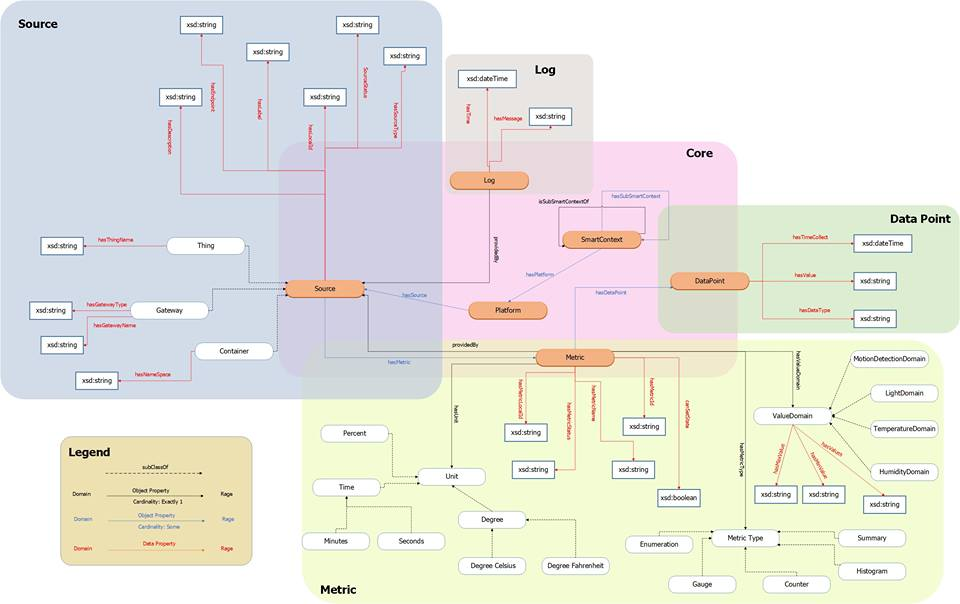
\includegraphics[scale=0.1]{ontology}
\caption{Cross-platform ontology.}
\end{figure}

- \textbf{Smart Context} is the root of the graph, which is a testbed implemeted the cross-platform system. \\
- \textbf{Platform} is \texttt{a multi-layer technology that enables straightforward provisioning, management, and automation of connected devices within the Internet of Things universe. It basically connects your hardware, however diverse, to the cloud by using flexible connectivity options, enterprise-grade security mechanisms, and broad data processing powers} \cite{platform}. \\
- \textbf{Source} is the device or component that generate the data. A \textbf{Source} might be a \textbf{Thing}, a \textbf{Gateway} or a \textbf{Container}. \\
- \textbf{Thing} is a device which is a set of sensors. \\
- \textbf{Gateway} is   .\\
- \textbf{Container} is   . \\
- \textbf{Log} is a service that collect the data generated from \textbf{Sources} and store it for future purpose. \\
- \textbf{Metric} is ... \\
- \textbf{Data Point} is generated when a \textbf{Metric} active. \\

\subsection{Resource Graph}

\begin{figure}[h]
\centering
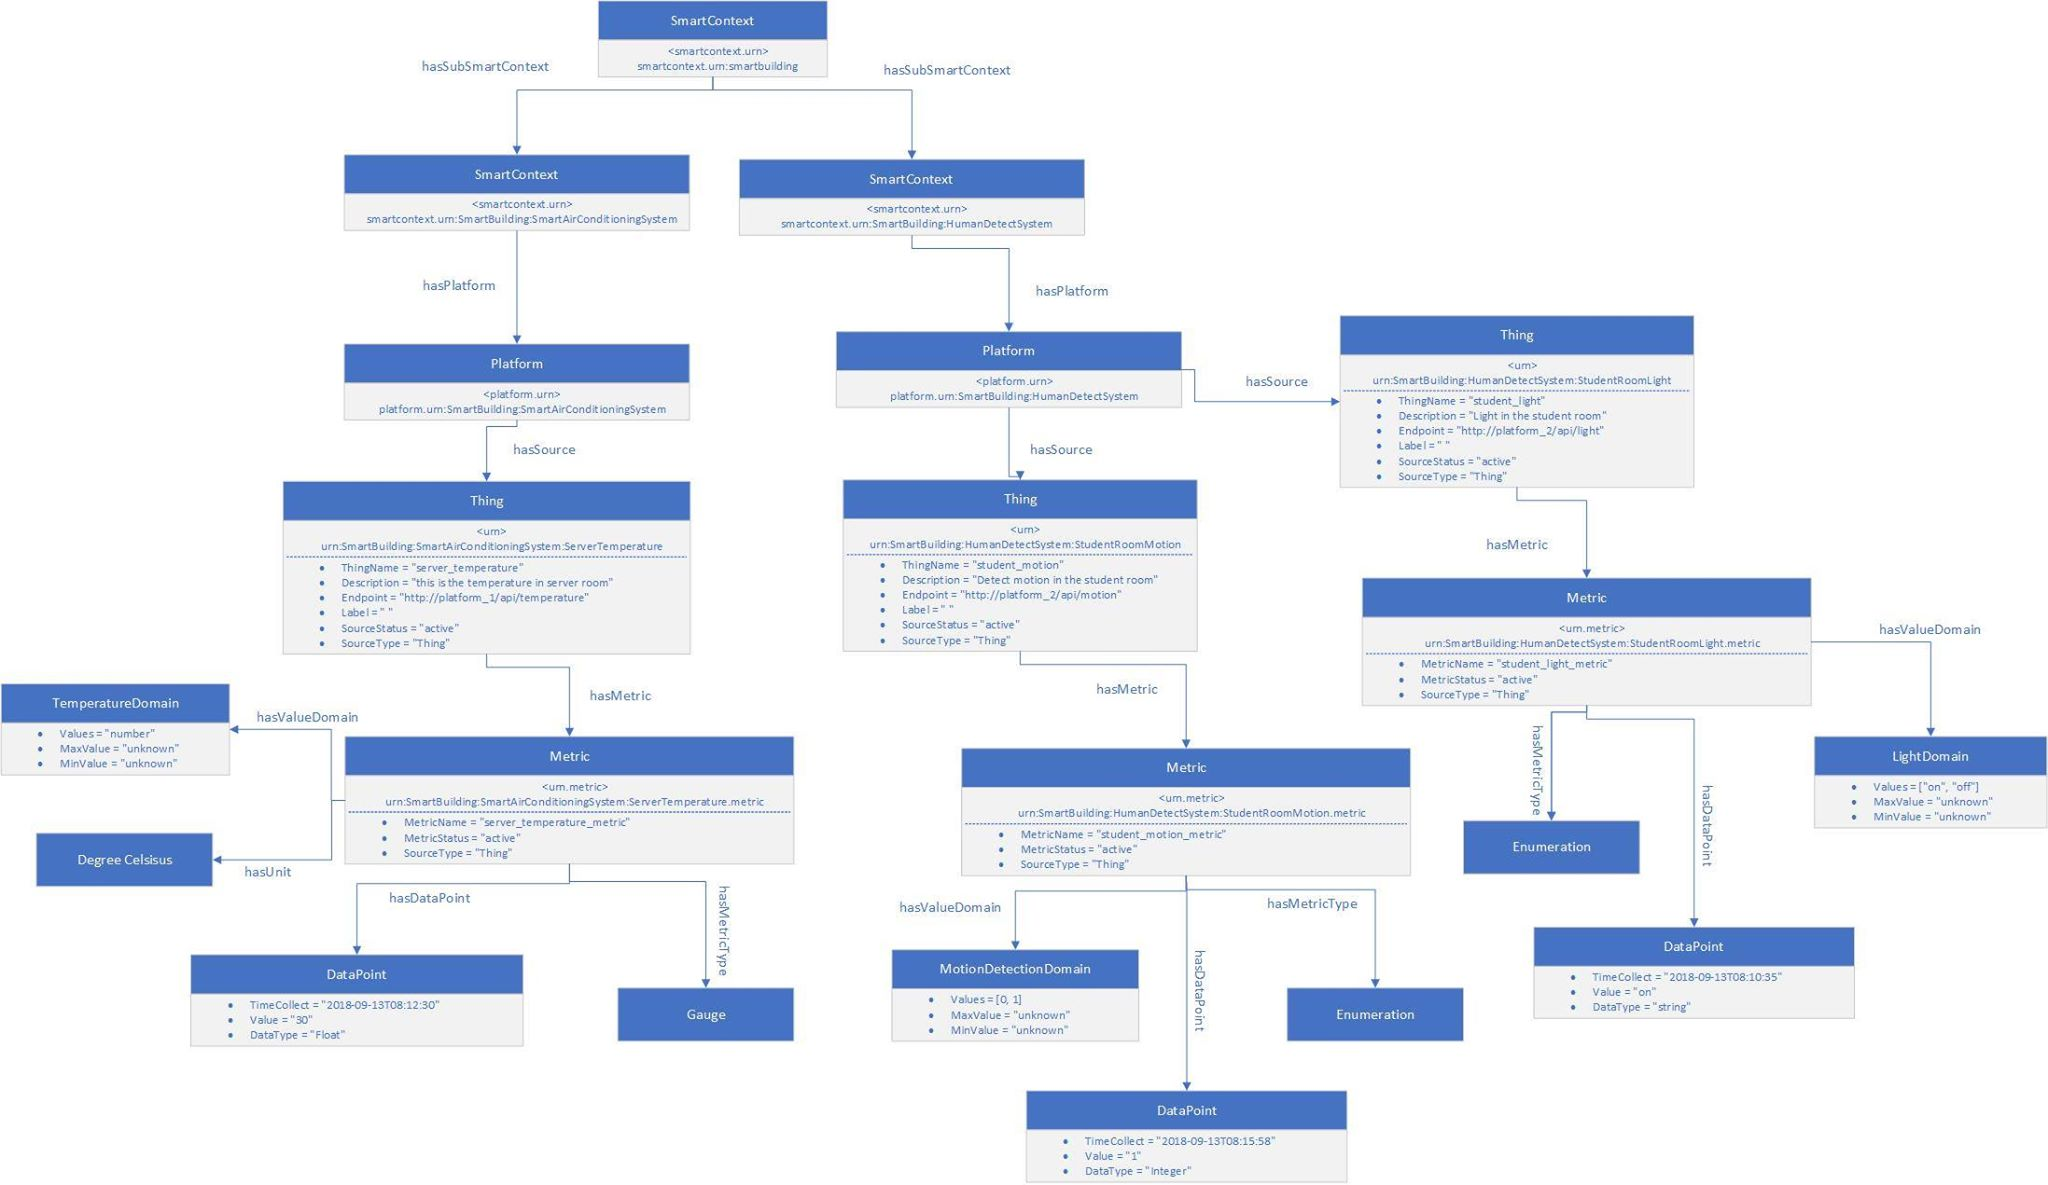
\includegraphics[scale=0.2]{resource_graph} 
\caption{Cross-platform ontology.}
\end{figure} 

Figure below show the format of resource graph.\\\\\\
1	smartcontext.um:SmartBuilding is a \texttt{Smart Context} \\
2	smartcontext.um:SmartBuilding:SmartAirconditionSystem is a \texttt{Smart Context} \\ 
3 	smartcontext.um:SmartBuilding:HumanDetecSystem is a \texttt{Smart Context} \\
4 	platform.um:SmartBuilding:SmartAirconditionSystem is a \texttt{Platform} \\
5 	platform.um:SmartBuilding:HumanDetecSystem is a \texttt{•}tt{Platform} \\
6 	urn:SmartBuilding:HumanDetecSystem:StudentRoomLight is a \texttt{Thing}\\
7		ThingName "student light" \\ 
8		Description "Light in the student room" \\
9		Endpoint "http://platform2/api/room" \\ 
10		Label "" \\
11		SourceStatus "active" \\
12		SourceType "Thing" \\
13 	urn:SmartBuilding:SmartAirconditionSystem:ServerTemperature is a \texttt{Thing} \\
14 	urn:SmartBuilding:HumanDetecSystem:StudentRoomMotion is a \texttt{Thing} \\
15 	



\section{Experiment}

\section{Conclusion}

\section{The References Section}\label{references}

\begin{thebibliography}{4}

\bibitem{platform} https://www.kaaproject.org/what-is-iot/

\end{thebibliography}

\end{document}
